\documentclass[convert]{standalone}

\usepackage{tikz}
\usetikzlibrary{backgrounds,angles,quotes,calc}
\usepgflibrary {shadings}

\begin{document}

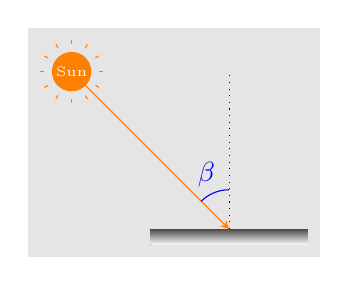
\begin{tikzpicture}[background rectangle/.style={fill=black!10}, show background rectangle,>=stealth]
  \fill[top color=black!70] (0,-0.2) rectangle (2,0);
  \coordinate (S) at (-1,2);
  \coordinate (I) at (1,0);
  \coordinate (N) at (1,2);

  \draw[dotted] (I) -- (N);
  \draw[->,orange] (S) -- (I);
  \fill[orange] (S) circle (0.25) node[white]{\tiny Sun};
  \foreach \a in {0,30,...,330}{
    \draw[orange] ($(S) + (\a:0.35)$) --($(S) + (\a:0.4)$);
  }
  \draw pic ["$\beta$",draw,blue,angle eccentricity=1.5]{angle=N--I--S};
\end{tikzpicture}

\end{document}

